\documentclass[11pt,a4paper]{article}

\usepackage[utf8]{inputenc}
\usepackage[T1]{fontenc}
\usepackage[english]{babel}
\usepackage{geometry}
\usepackage{amsmath}
\usepackage{amssymb}
\usepackage{booktabs}
\usepackage{tabularx}
\usepackage{array}
\usepackage{enumitem}
\usepackage{xcolor}
\usepackage{graphicx}
\graphicspath{{./}{../}}
\usepackage{float}
\usepackage{caption}
\usepackage{microtype}
\usepackage{hyperref}

\geometry{margin=2.45cm}
\setlength{\parindent}{0pt}
\setlength{\parskip}{0.52em}
\setlist[itemize]{leftmargin=*, itemsep=0.20em, topsep=0.30em}
\setlist[enumerate]{leftmargin=*, itemsep=0.25em, topsep=0.30em}
\captionsetup{font=small, labelfont=bf}
\hypersetup{
    colorlinks=true,
    linkcolor=blue!55!black,
    urlcolor=blue!55!black,
    citecolor=blue!55!black,
    pdftitle={EEG Causal Graphs for Three-Class Classification},
    pdfauthor={Michele Arrigoni}
}

\newcommand{\R}{\mathbb{R}}
\newcommand{\methodset}{\{G,L,P\}}

\title{
    \textbf{EEG Causal Graphs for Three-Class Classification}\\[0.35em]
    \large Preprocessing, directed connectivity estimation, and baseline
    classification for AD, CN, and FTD
}
\author{Michele Arrigoni}
\date{September 2026}

\begin{document}

\maketitle

\begin{abstract}
This project builds a graph-based representation of resting-state EEG
recordings for three-class classification among Alzheimer's disease (AD),
healthy controls (CN), and frontotemporal dementia (FTD). Each subject is
represented by a graph whose nodes are the 19 EEG channels, whose node
attributes describe local spectral and statistical activity, and whose edges
encode directed connectivity estimated from time-series methods.

The pipeline combines filtering over a 0.5--40 Hz passband, resampling to
100 Hz, epoch quality control, and stationarity testing. Spectral features
are computed before differencing, while connectivity is estimated using
Granger causality, VARLiNGAM, and PCMCI. Each method produces separate directed
and symmetric graph representations. The current exports contain 87 OpenNeuro
and 85 BrainLat subjects. Connectivity is summarized separately for each
dataset and clinical class. A compact MLP is trained and evaluated independently
within each dataset.
% BEGIN AUTO MLP_HEADLINE
On OpenNeuro, VARLiNGAM achieves the highest observed test balanced accuracy (0.605).
On BrainLat, Granger and VARLiNGAM tie for the highest observed test balanced accuracy (0.821).
% END AUTO MLP_HEADLINE
These single-split results do not measure cross-dataset generalization.
\end{abstract}

\tableofcontents
\newpage

\section{Objective and Data Representation}

\subsection{Project objective}

The objective is to transform multichannel EEG recordings into homogeneous
graph samples suitable for graph neural models and for simpler subject-level
classification baselines. For each subject $s$, the recording is represented
as a graph:
\[
    G_s=(V_s,X_s,A_s,y_s),
\]
where $V_s$ is the fixed set of EEG electrodes, $X_s$ contains node features,
$A_s$ is a weighted adjacency matrix, and $y_s\in\{0,1,2\}$ is the clinical
label. Label 0 denotes CN, label 1 denotes AD, and label 2 denotes FTD.

The term causal is used in the statistical sense of the adopted estimators:
Granger, VARLiNGAM, and PCMCI provide evidence that the past or structural
state of one channel helps explain another channel under the model
assumptions. In this report, an edge therefore means a model-based
directional dependence in the observed EEG channels. It does not prove a
direct physiological pathway, because scalp EEG is affected by volume
conduction, reference choices, latent neural sources, and estimator
assumptions.

\subsection{Processed datasets}

The current processed exports contain 87 OpenNeuro subjects and 85
BrainLat subjects. OpenNeuro subject \texttt{sub-086} and BrainLat subject
\texttt{sub-078} are excluded from the analyses because their preprocessing
outputs are not compatible with the shared-duration exports used for the
report. All connectivity summaries and MLP experiments in this report are
computed separately by dataset. The 172 analyzed subjects are not pooled for
classification because OpenNeuro and BrainLat differ in cohort composition,
acquisition conditions, retained duration, and electrode geometry; pooling
them would make dataset identity a potential confounder.

% BEGIN AUTO INVENTORY
\begin{table}[H]
\centering\small
\begin{tabular}{llllll}
\toprule
Dataset & CN & AD & FTD & Total & Epochs/subject \\
\midrule
OpenNeuro & 29 & 36 & 22 & 87 & 61 \\
BrainLat & 32 & 35 & 18 & 85 & 28 \\
\bottomrule
\end{tabular}
\caption{Current processed exports, analyzed separately by dataset.}
\end{table}

% END AUTO INVENTORY

BrainLat electrodes are mapped to the 19 canonical channels by selecting
available electrodes nearest to normalized standard-1020 montage coordinates,
without reusing an electrode. This harmonizes channel names and order but
does not establish identical acquisition geometry across datasets.
The coordinates are used only to choose the closest available BrainLat sensor
for each target 10--20 label; they are not used as spatial features in the
classifier.

All graphs share the same 19-channel order:
\[
\begin{split}
&\mathrm{Fp1,\ Fp2,\ F3,\ F4,\ C3,\ C4,\ P3,\ P4,\ O1,\ O2,}\\
&\mathrm{F7,\ F8,\ T3,\ T4,\ T5,\ T6,\ Fz,\ Cz,\ Pz}.
\end{split}
\]
This order is enforced before feature extraction and adjacency construction,
so the same row and column always refer to the same electrode.
Equivalently, every feature vector and adjacency matrix can be read as if it
used the same fixed electrode layout.

\section{Preprocessing Pipeline}

\subsection{Filtering, resampling, and epochs}

Recordings are loaded from EEGLAB files with MNE, restricted to the canonical
19 channels, band-pass filtered between 0.5 and 40 Hz, notch-filtered at 50 Hz,
and resampled to 100 Hz. The Nyquist frequency is the highest frequency that
can be represented after sampling without aliasing, and is one half of the
sampling rate:
\[
    f_N=\frac{100}{2}=50\ \mathrm{Hz},
\]
which preserves the delta, theta, alpha, beta, and low-gamma ranges used by
the node features.

The continuous signal is split into non-overlapping 5-second epochs:
\[
    L=f_sT=100\cdot5=500
\]
samples per epoch before stationarity differencing. OpenNeuro outputs are
cropped to 61 valid epochs per subject in the current processed dataset, while
BrainLat outputs are cropped to 28 valid epochs per subject. Within each
dataset the pipeline takes the first shared-minimum number of accepted
epochs, corresponding to 305 and 140 seconds of selected data respectively
before differencing; these windows need not be contiguous in the original
recording because rejected epochs are skipped. This choice gives all subjects
within a dataset the same number of epochs, preventing recording duration from
becoming an unintended classifier signal.

\subsection{Quality control}

Epochs are discarded when they contain non-finite values, extreme amplitudes,
or nearly flat channels. The amplitude threshold is:
\[
    150\times10^{-6}\ \mathrm{V},
\]
which corresponds to 150 microvolts in the unit convention normally returned
by MNE. Amplitude screening is performed before channel standardization.

Accepted epochs are standardized channel by channel:
\[
    z_{i,t}=\frac{x_{i,t}-\mu_i}{\sigma_i+\varepsilon}.
\]
Here $x_{i,t}$ is the sample of channel $i$ at time $t$, $\mu_i$ and
$\sigma_i$ are the mean and standard deviation of that channel within the
epoch, and $\varepsilon$ is a small constant that prevents division by zero.
This normalization reduces scale differences across channels and subjects
before causal estimation.

\subsection{Stationarity handling}

Granger-style autoregressive inference assumes approximately stationary time
series. Each channel is tested using ADF and KPSS:
\[
    p_{\mathrm{ADF}}\leq0.05,\qquad p_{\mathrm{KPSS}}>0.05.
\]
When one or more channels fail the criterion, the epoch is differenced along
time:
\[
    \Delta X_t=X_t-X_{t-1},
\]
up to two times. Differenced epochs are used for causal estimation.
At the limit the epoch is retained even if it still fails the tests, to avoid
discarding too much data after quality control. The stationarity checks are
therefore a preprocessing heuristic rather than a guarantee that every final
series is perfectly stationary.

Spectral node features are computed from standardized epochs before
differencing. This preserves low-frequency content, particularly in the
delta band, which can be distorted by the high-pass effect of differencing.
The pipeline retains separate pre-differencing and stationarity-processed
representations for feature extraction and connectivity estimation,
respectively.

\section{Node Features}

For each channel, the feature vector has eight components:
\[
    x_i =
    [P_\delta,P_\theta,P_\alpha,P_\beta,P_\gamma,\mu,\sigma,\sigma^2].
\]
The five spectral features are band powers of the Z-scored signals estimated
with Welch's method~\cite{welch1967} over:
\[
\delta:0.5\text{--}4,\quad
\theta:4\text{--}8,\quad
\alpha:8\text{--}13,\quad
\beta:13\text{--}24,\quad
\gamma:24\text{--}40\ \mathrm{Hz}.
\]
Mean, standard deviation, and variance are computed over the accepted
pre-differencing samples of the channel.

Stacking the eight features for all 19 channels yields the subject-level
node-feature matrix:
\[
    X_s\in\R^{19\times8}.
\]

\section{Directed Connectivity Estimation}

\subsection{Common representation and temporal aggregation}

Connectivity is estimated independently for each subject and epoch from the
stationarity-processed signals. With $N=19$ channels, each method produces
an $N\times N$ directed matrix with $N(N-1)=342$ possible off-diagonal
connections. Throughout this section, $W^{(e,m)}_{ij}$ denotes the raw
epoch-level weight from source $j$ to target $i$ for method $m$.
Self-connections are excluded from the resulting connectivity matrices.
Autoregressive self-history can nevertheless be used internally by the
estimators when predicting a channel: a target channel may use its own past
as a baseline predictor, but the saved graph does not store self-edges on the
diagonal.

The subject-level matrix is formed as
\[
    W_s^{(m)}=\frac{1}{|\mathcal E_s^{(m)}|}
    \sum_{e\in\mathcal E_s^{(m)}} W_s^{(e,m)},
\]
where $\mathcal E_s^{(m)}$ is the set of epochs included in the aggregation.
Granger and VARLiNGAM average the supplied epochs; PCMCI excludes epochs
whose estimation fails and returns a zero matrix if none succeeds.
Consequently, a zero PCMCI output must be interpreted together with processing
diagnostics. Averaging yields a static summary and removes information about
when individual connections occur within the recording.

\subsection{Granger causality}

Pairwise Granger causality measures whether past values of a source channel
improve prediction of a target channel beyond the target's own past:
\[
    Y_t =
    \sum_{r=1}^{p}a_rY_{t-r}
    +
    \sum_{r=1}^{p}b_rX_{t-r}
    +\eta_t.
\]
The null hypothesis is:
\[
    H_0:b_1=b_2=\cdots=b_p=0.
\]
For each ordered pair of channels and each epoch, autoregressive orders
$p\in\{1,2,3,4\}$ are tested using the residual-sum-of-squares F test
implemented by \texttt{statsmodels}. At 100 Hz, these lags correspond to
10--40 ms of past activity. This range is important because Granger causality
can only detect predictive effects that occur within the tested delay window:
short windows emphasize fast EEG interactions, while longer windows would
increase model complexity and computational cost. Each order tests the joint
contribution of all source lags from 1 to $p$, rather than testing only the
individual lag $p$.

For every source--target pair, the implementation keeps the smallest finite
p-value across the tested orders:
\[
    \pi_{ij}^{(e)}=\min_{p\in\{1,2,3,4\}}\pi_{ij,p}^{(e)}.
\]
The candidate p-values are then corrected across all ordered pairs in the
epoch using Benjamini--Hochberg false-discovery-rate control. The raw
epoch-level weight is:
\[
    W_{ij}^{(e,G)}=
    \begin{cases}
    -\log_{10}\left(\max(\pi_{ij}^{(e)},10^{-12})\right),
    & \text{if the FDR-corrected test is significant},\\
    0, & \text{otherwise}.
    \end{cases}
\]
Subject-level Granger adjacency is the average across accepted epochs.

A smaller p-value gives a larger positive score after the
$-\log_{10}(\cdot)$ transformation. This score measures statistical evidence
against the no-predictive-effect null hypothesis; it is neither a probability
of causation nor the magnitude of a regression coefficient. The analysis is
pairwise, so it does not condition on the other 17 channels. Indirect paths
and common drivers can therefore contribute to the detected relationships.
The configured significance level is $\alpha=0.01$.

\subsection{VARLiNGAM}

VARLiNGAM~\cite{varlingamdocs} is a vector autoregressive extension of
LiNGAM. It models multivariate time series and estimates instantaneous and
lagged structural effects:
\[
    x(t)=B_0x(t)+B_1x(t-1)+\cdots+B_px(t-p)+e(t).
\]
The implementation configures a maximum order of four samples, uses BIC
for order selection, and enables coefficient pruning. BIC penalizes overly
complex autoregressive models, while pruning suppresses coefficients that the
fitted VARLiNGAM model regards as weak. Let $p_e$ denote the number of lag
matrices returned for epoch $e$. The instantaneous matrix $B_0$ participates
in the model but is excluded from the stored connectivity aggregation because
lagged effects are easier to compare with Granger and PCMCI, which are also
stored as positive-lag directed graphs. The lagged matrices are averaged in
absolute value:
\[
    W_{ij}^{(e,L)} =
    \begin{cases}
    \displaystyle\frac{1}{p_e}\sum_{\tau=1}^{p_e}
    \left|B_{\tau,ij}^{(e)}\right|, & p_e>0,\\
    0, & p_e=0.
    \end{cases}
\]
This produces a directed non-negative adjacency matrix in the same
\texttt{target, source} orientation used by the other methods.

Unlike the Granger score, this weight summarizes fitted structural
coefficient magnitudes in a multivariate model. Taking absolute values is
appropriate here because the downstream graph representation uses
non-negative edge strengths; it prevents opposite signs across lags from
cancelling. The cost is that the saved graph no longer distinguishes
excitatory-like and inhibitory-like signed effects. Averaging also removes
the individual delay associated with each coefficient. Interpretation depends
on the linear structural model and its assumptions, including independent
non-Gaussian innovations and an acyclic instantaneous structure; the
aggregated lagged graph is not required to be acyclic.

\subsection{PCMCI}

PCMCI~\cite{runge2019} identifies lagged dependencies in multivariate time
series through a parent-selection stage followed by conditional-independence
testing. The acronym refers to the combination of PC-style parent selection
and momentary conditional independence testing. This project uses the ParCorr
test. For a candidate source $j$ and target $i$, PCMCI tests whether:
\[
    X_{t-\tau}^{(j)}
    \not\!\perp\!\!\!\perp
    X_t^{(i)}
    \mid \mathbf{Z},
\]
where $\mathbf{Z}$ contains selected lagged parents. The notation reads as:
``the source channel $j$ at lag $\tau$ is not conditionally independent of
the current target channel $i$, given the selected conditioning set
$\mathbf{Z}$.'' The parent-selection stage reduces the conditioning sets, and
the momentary conditional independence stage evaluates candidate links given
the selected variables. With ParCorr, dependence is measured through the
correlation of residuals after linear conditioning. The implementation uses
analytic significance tests~\cite{tigramitedocs} and sets both the
parent-selection threshold and the final edge threshold to 0.01 through the
shared project configuration.

For a source--target pair, define the significant positive-lag set as
\[
    \mathcal T_{ij}^{(e)}=
    \{\tau\in\{1,2,3,4\}:p_{j,i,\tau}^{(e)}<0.01\}.
\]
The raw epoch-level weight is
\[
    W_{ij}^{(e,P)}=
    \begin{cases}
    \displaystyle\frac{1}{|\mathcal T_{ij}^{(e)}|}
    \sum_{\tau\in\mathcal T_{ij}^{(e)}}
    |\rho_{j,i,\tau}^{(e)}|, & |\mathcal T_{ij}^{(e)}|>0,\\
    0, & \text{otherwise},
    \end{cases}
\]
where $\rho$ is the partial-correlation value returned by PCMCI. Only
significant lags enter this mean: a link with one strong significant lag
can therefore have a larger weight than a link with several weaker ones.
Lag-zero links and self-connections are excluded from the stored graph.

Multivariate conditioning addresses dependencies explained by the selected
observed variables, but does not establish immunity to unobserved
confounding. ParCorr targets linear conditional relationships, and taking
absolute values discards their signs. The final filtering uses the returned
p-values directly, without false-discovery-rate adjustment.

\section{Connectivity Results}

\subsection{Dataset-specific averaging and display rules}

For each dataset $d$, method $m$ and class $c$, the saved normalized directed
matrices are averaged with equal weight for every subject:
\[
\overline A^{(d,m,c)}=\frac{1}{N_{d,c}}
\sum_{s\in d:y_s=c}A_{s,\mathrm{normal}}^{(m)}.
\]
No average mixes OpenNeuro and BrainLat subjects. Matrices describe relative
connectivity after subject-specific normalization, not absolute physiological
coupling strength. Heatmaps display every entry with a common scale across
classes within each dataset and method.

For network visualization, a separate threshold is calculated for every
dataset and method from the off-diagonal entries of its three class means:
\[
q_{d,m}=Q_{0.80}\left(\{\overline A_{ij}^{(d,m,c)}:
 i\ne j,\ c\in\{\mathrm{CN,AD,FTD}\}\}\right).
\]
The percentile includes all $3\times342=1026$ values, including zeros.
Only weights strictly above $q_{d,m}$ are drawn. The threshold is shared
across classes within a dataset and method; it does not impose a fixed density
on each class. Color scales and thresholds can differ between datasets, so
visual edge counts cannot establish an absolute between-dataset difference.
Consequently, $q_{d,m}$ should be read as a display cutoff that selects the
upper tail of the class-average matrices, not as an inferential threshold.

For each displayed graph, $K$ is the number of retained directed edges,
$d=K/342$ its density, and $\overline w$ the mean retained normalized weight.
Reciprocal links count as two edges. Thresholding is descriptive, is not a
statistical significance test, and is never applied to classifier inputs.
The figures summarize all exported subjects, including held-out subjects,
solely for descriptive analysis; these averages are not training features.

% BEGIN AUTO CONNECTIVITY
\subsection{OpenNeuro}
This dataset contains 87 subjects (29 CN, 36 AD and 22 FTD), with 61 retained epochs per subject.
\begin{figure}[H]
\centering
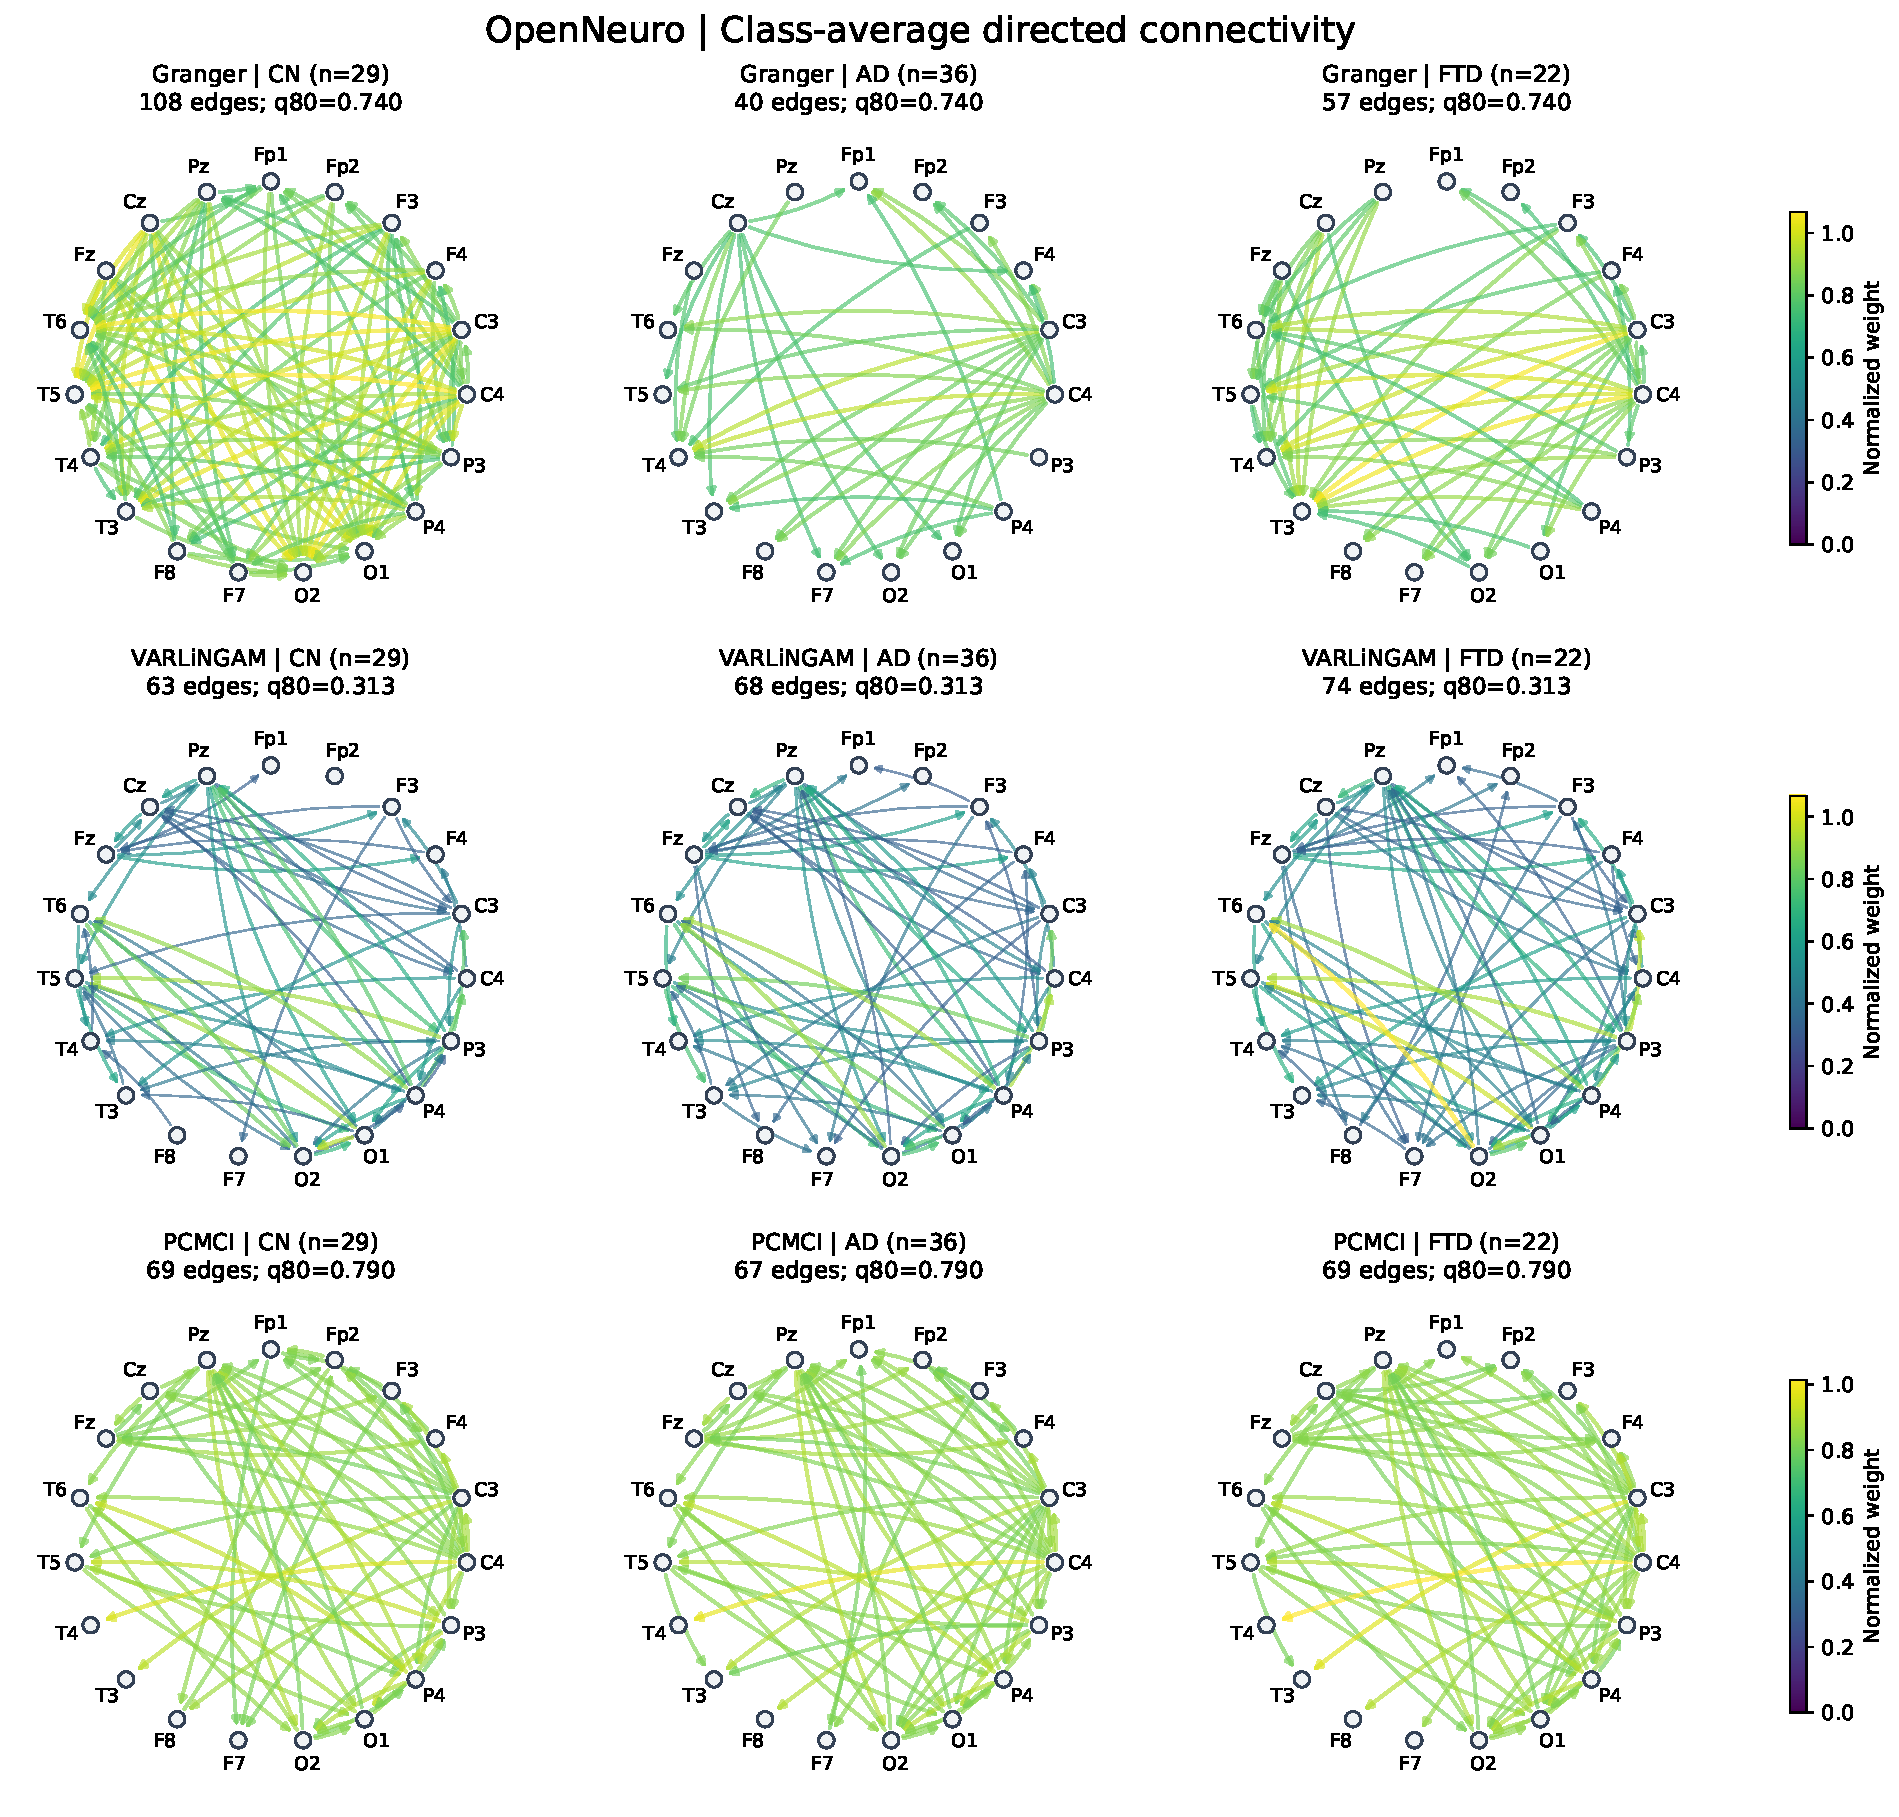
\includegraphics[width=\textwidth,height=0.70\textheight,keepaspectratio,page=1]{figures/connectivity_networks.pdf}
\caption{OpenNeuro: class-average directed networks. Arrows run from source to target; color and width encode normalized weight. Circular positions indicate channel order, not anatomy. Scales and thresholds are shared across classes within each method.}
\end{figure}
\begin{figure}[H]
\centering
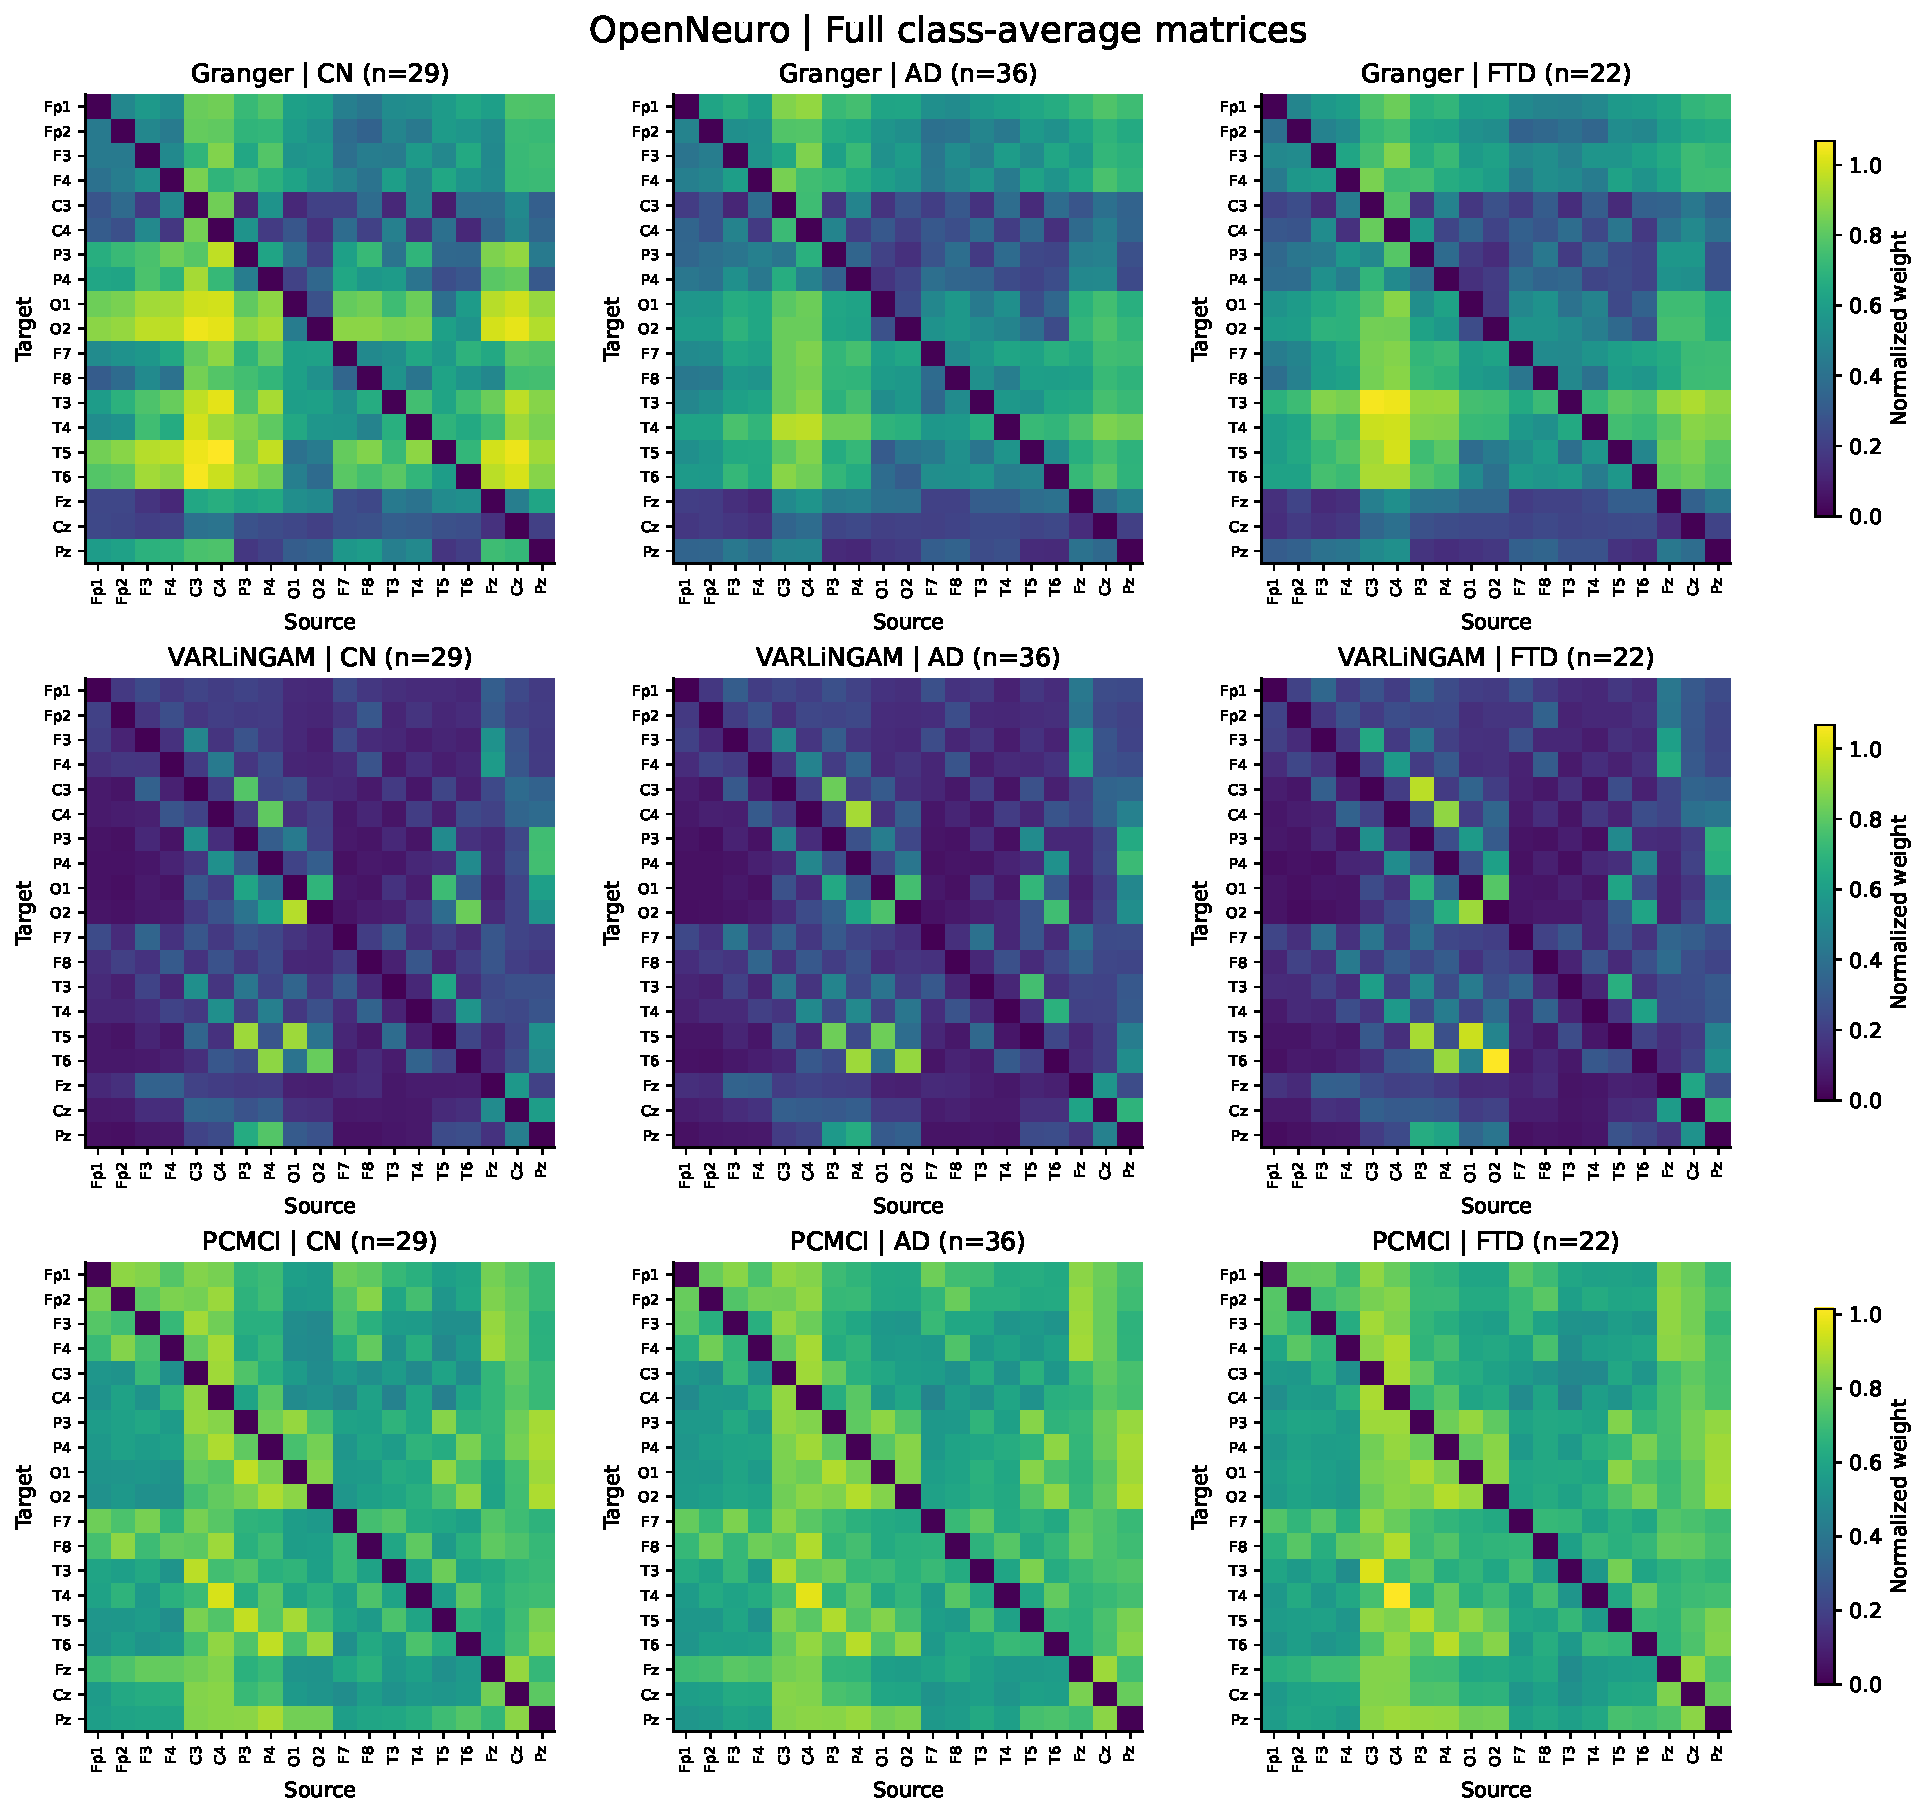
\includegraphics[width=\textwidth,height=0.70\textheight,keepaspectratio]{figures/connectivity_openneuro_heatmaps.pdf}
\caption{OpenNeuro: unthresholded class-average matrices. Rows are targets, columns are sources; each method shares its color scale across classes.}
\end{figure}
\begin{figure}[H]
\centering
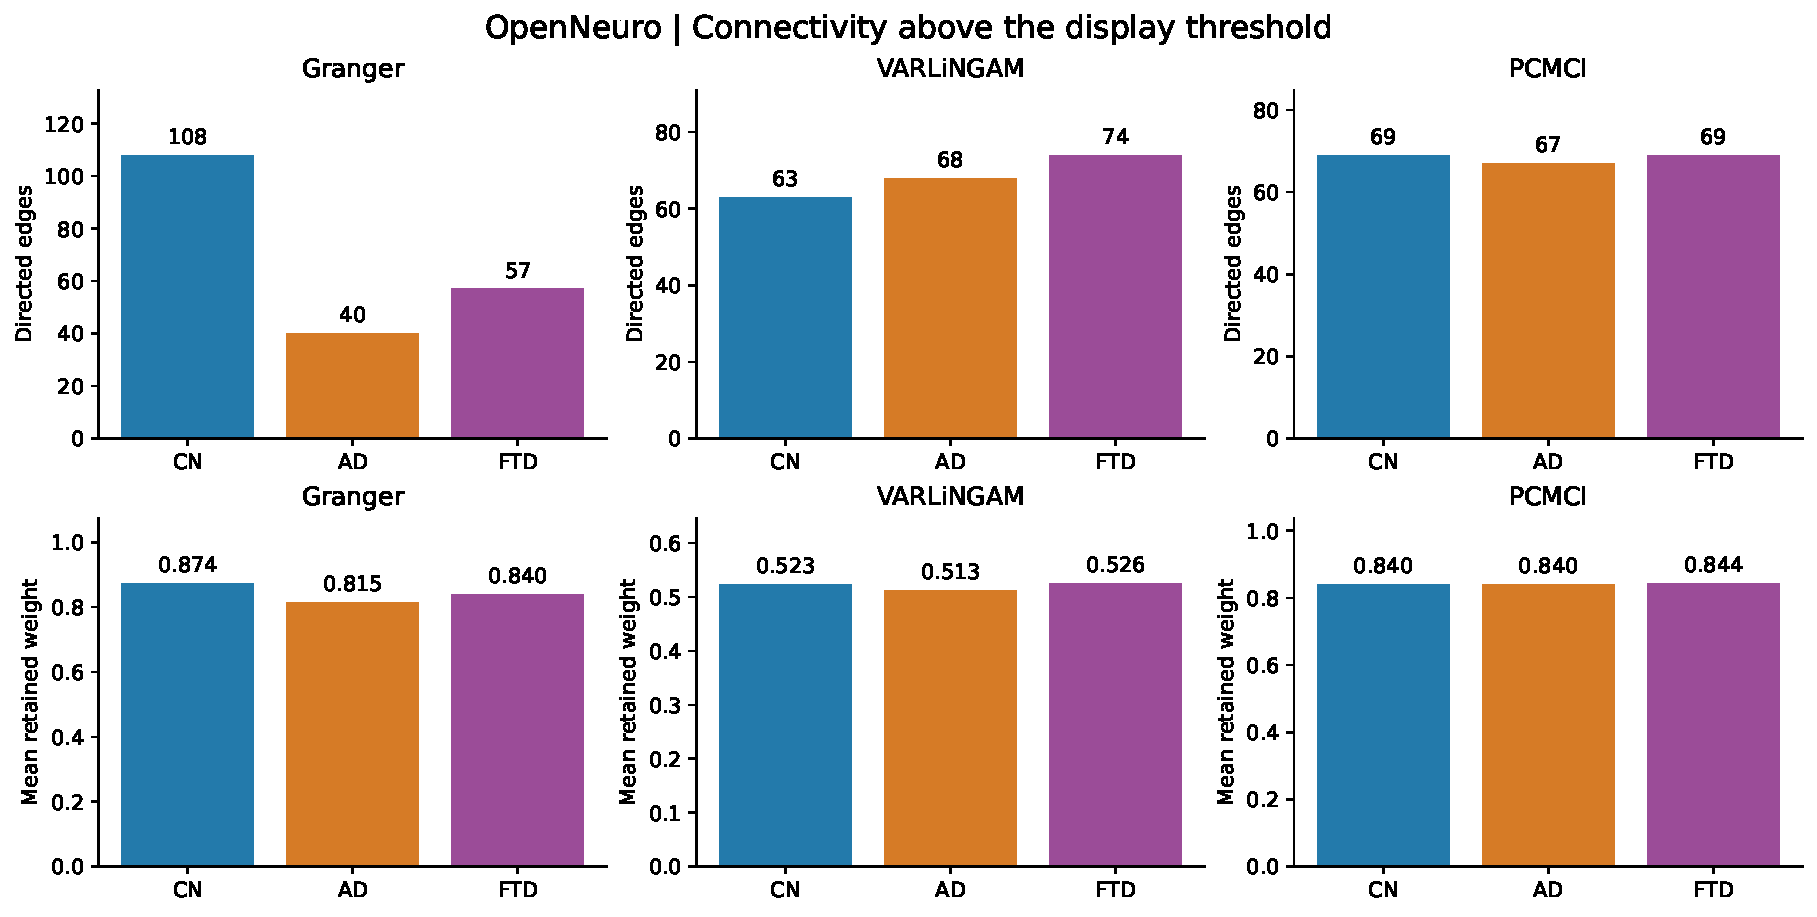
\includegraphics[width=\textwidth,height=0.40\textheight,keepaspectratio,page=1]{figures/connectivity_summary.pdf}
\caption{OpenNeuro: edge counts and mean retained weights above the dataset- and method-specific 80th percentile.}
\end{figure}
\begin{table}[H]
\centering\small
\begin{tabular}{llllll}
\toprule
Method & Class & $q_{d,m}$ & Edges & Density & Mean weight \\
\midrule
Granger & CN & 0.740 & 108 & 0.316 & 0.874 \\
Granger & AD & 0.740 & 40 & 0.117 & 0.815 \\
Granger & FTD & 0.740 & 57 & 0.167 & 0.840 \\
VARLiNGAM & CN & 0.313 & 63 & 0.184 & 0.523 \\
VARLiNGAM & AD & 0.313 & 68 & 0.199 & 0.513 \\
VARLiNGAM & FTD & 0.313 & 74 & 0.216 & 0.526 \\
PCMCI & CN & 0.790 & 69 & 0.202 & 0.840 \\
PCMCI & AD & 0.790 & 67 & 0.196 & 0.840 \\
PCMCI & FTD & 0.790 & 69 & 0.202 & 0.844 \\
\bottomrule
\end{tabular}
\caption{OpenNeuro: thresholded class-average connectivity statistics.}
\end{table}

\subsection{BrainLat}
This dataset contains 85 subjects (32 CN, 35 AD and 18 FTD), with 28 retained epochs per subject.
\begin{figure}[H]
\centering
\includegraphics[width=\textwidth,height=0.70\textheight,keepaspectratio,page=2]{figures/connectivity_networks.pdf}
\caption{BrainLat: class-average directed networks. Arrows run from source to target; color and width encode normalized weight. Circular positions indicate channel order, not anatomy. Scales and thresholds are shared across classes within each method.}
\end{figure}
\begin{figure}[H]
\centering
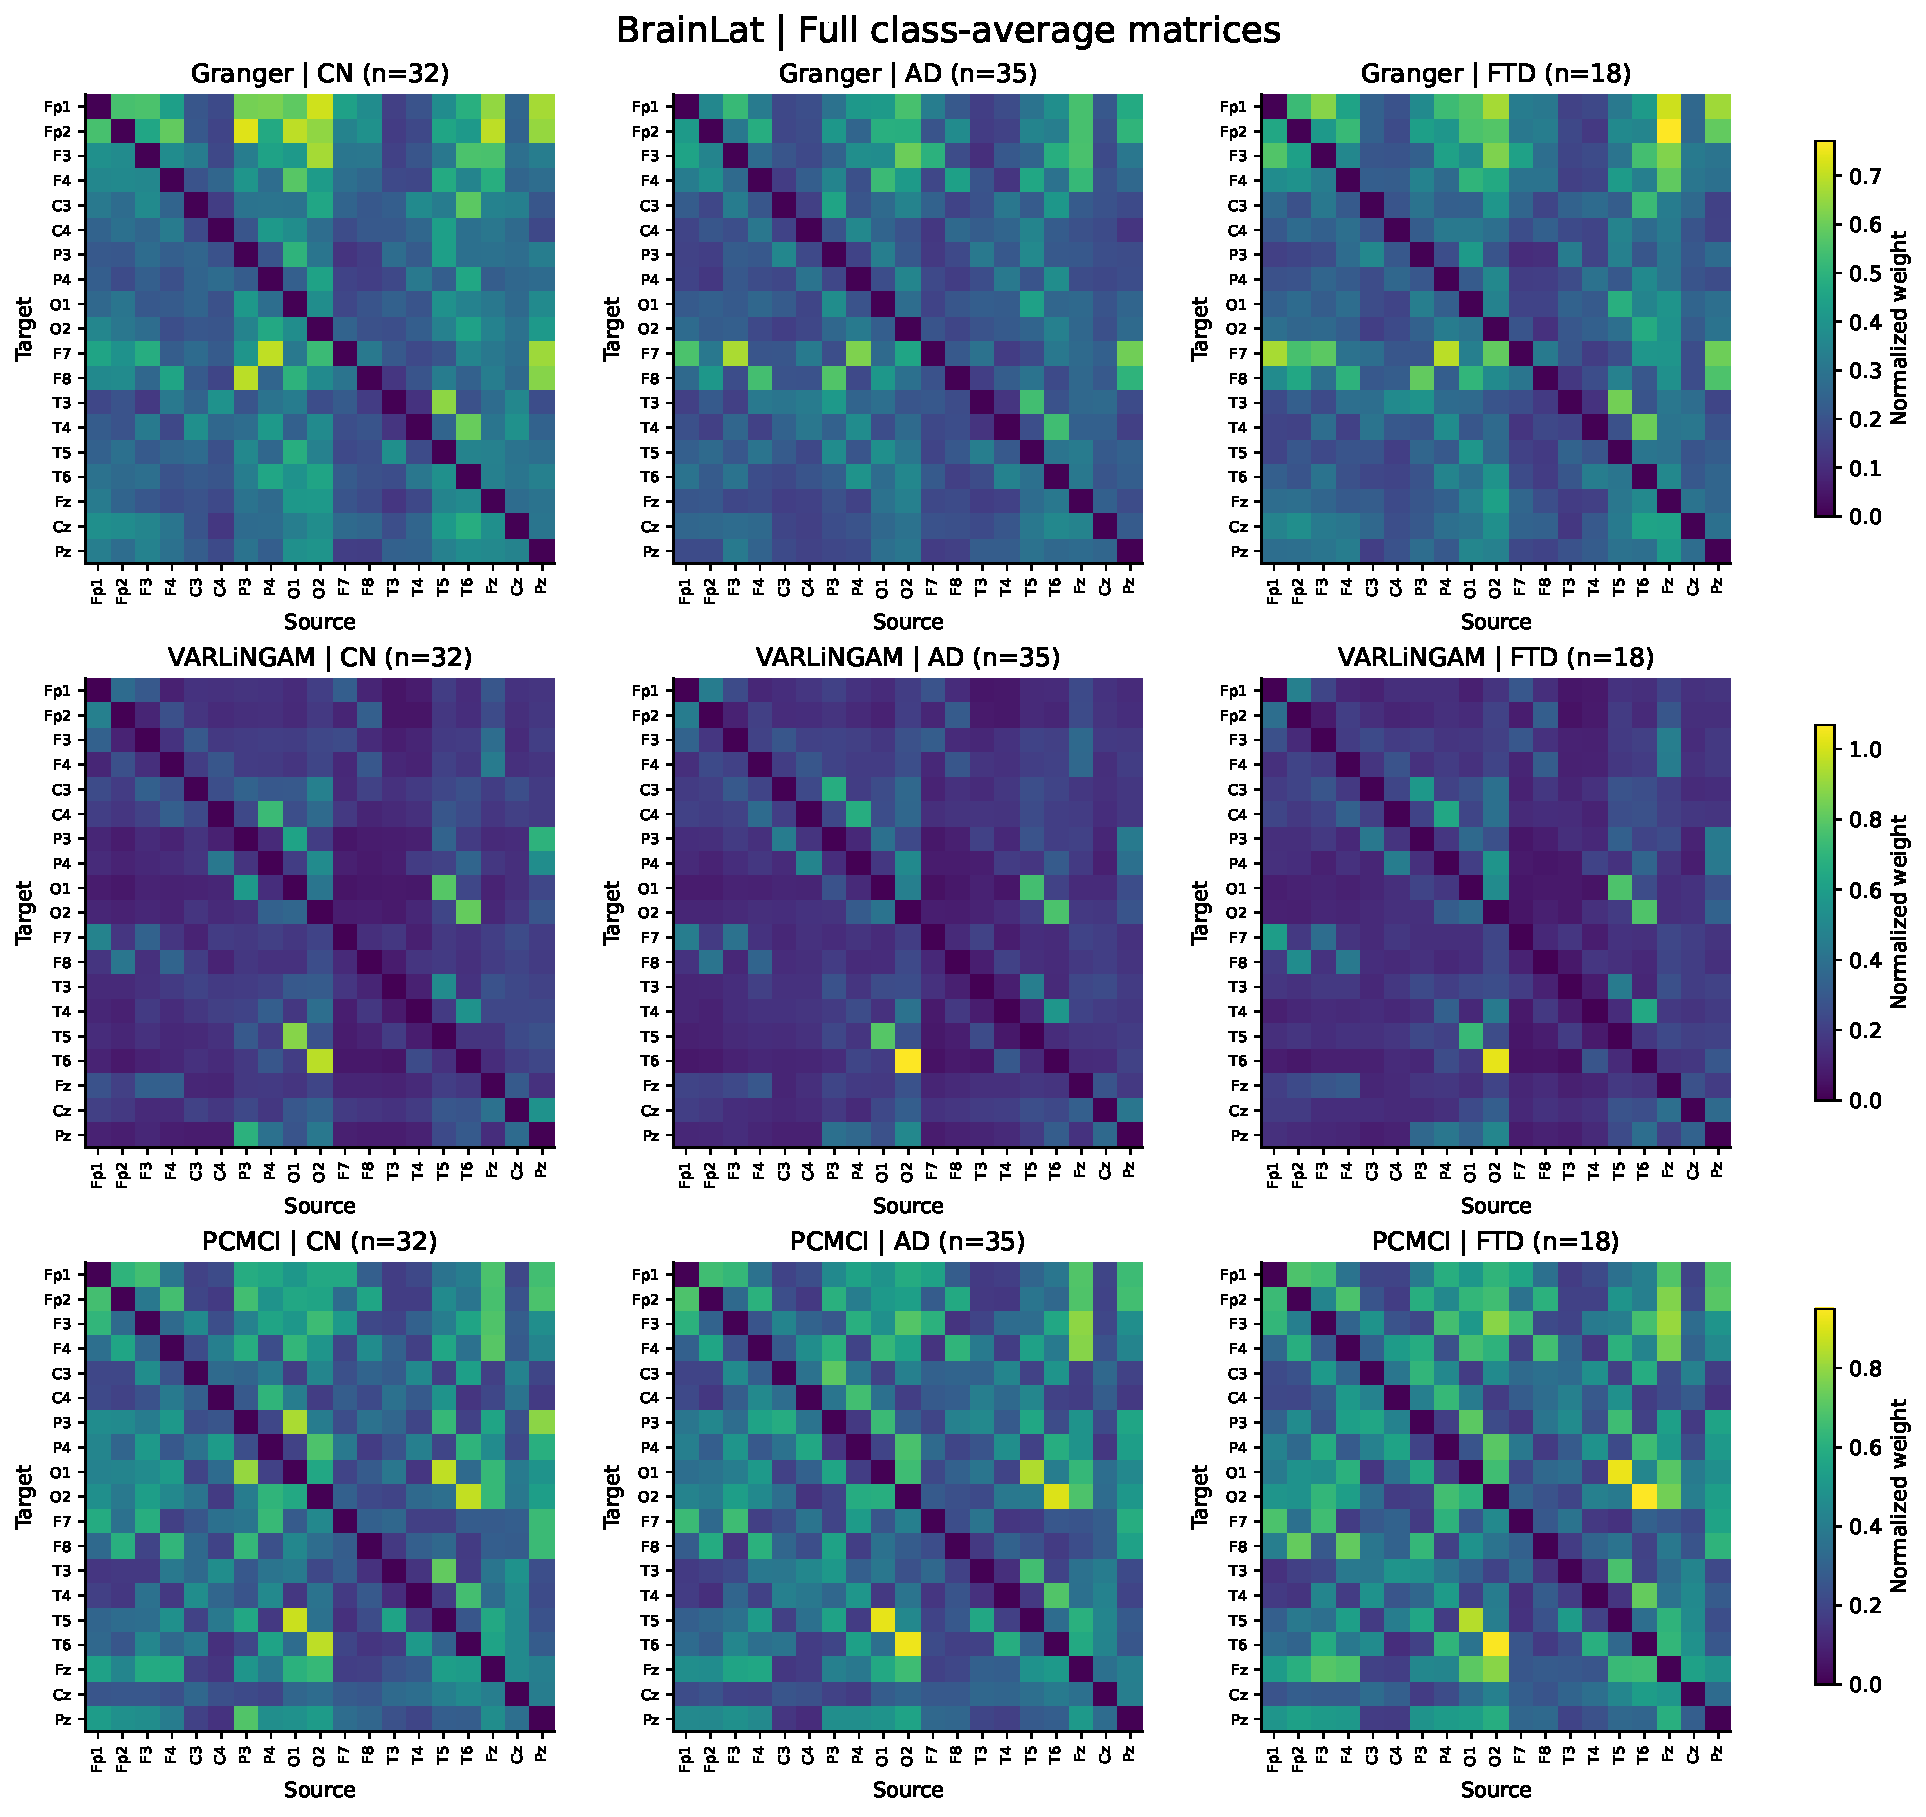
\includegraphics[width=\textwidth,height=0.70\textheight,keepaspectratio]{figures/connectivity_brainlat_heatmaps.pdf}
\caption{BrainLat: unthresholded class-average matrices. Rows are targets, columns are sources; each method shares its color scale across classes.}
\end{figure}
\begin{figure}[H]
\centering
\includegraphics[width=\textwidth,height=0.40\textheight,keepaspectratio,page=2]{figures/connectivity_summary.pdf}
\caption{BrainLat: edge counts and mean retained weights above the dataset- and method-specific 80th percentile.}
\end{figure}
\begin{table}[H]
\centering\small
\begin{tabular}{llllll}
\toprule
Method & Class & $q_{d,m}$ & Edges & Density & Mean weight \\
\midrule
Granger & CN & 0.370 & 89 & 0.260 & 0.482 \\
Granger & AD & 0.370 & 50 & 0.146 & 0.469 \\
Granger & FTD & 0.370 & 66 & 0.193 & 0.498 \\
VARLiNGAM & CN & 0.250 & 76 & 0.222 & 0.390 \\
VARLiNGAM & AD & 0.250 & 63 & 0.184 & 0.389 \\
VARLiNGAM & FTD & 0.250 & 66 & 0.193 & 0.395 \\
PCMCI & CN & 0.542 & 65 & 0.190 & 0.638 \\
PCMCI & AD & 0.542 & 64 & 0.187 & 0.632 \\
PCMCI & FTD & 0.542 & 76 & 0.222 & 0.662 \\
\bottomrule
\end{tabular}
\caption{BrainLat: thresholded class-average connectivity statistics.}
\end{table}

% END AUTO CONNECTIVITY

The circular plots show the identity and direction of the strongest displayed
links; the heatmaps retain weaker connections that the network display omits.
In the updated OpenNeuro summary, Granger shows the clearest class separation
in displayed edge count: CN retains 108 directed edges above the shared
OpenNeuro Granger threshold, compared with 40 for AD and 57 for FTD.
VARLiNGAM is more even and increases mildly from CN to FTD (63, 68 and 74
edges), while PCMCI is almost class-balanced in retained edge count (69, 67
and 69 edges). Mean retained weights vary much less than edge counts within
each OpenNeuro method, especially for PCMCI.

In BrainLat, the updated plots show a similar Granger ordering in which CN
has the largest displayed edge count (89), AD the smallest (50), and FTD is
intermediate (66). VARLiNGAM again varies moderately across classes, with CN
retaining 76 edges and AD/FTD retaining 63 and 66. PCMCI differs from this
pattern: FTD has the largest displayed count (76) and also the largest mean
retained weight (0.662). Across both datasets, VARLiNGAM has lower numerical
mean retained weights than Granger or PCMCI because its saved values are
normalized structural coefficient magnitudes rather than transformed p-value
evidence or partial-correlation magnitudes.

A larger retained-edge count does not establish a disease effect. Group
comparisons would require subject-level inference, multiplicity control and
sensitivity analysis across thresholds. The different estimators have distinct
weight definitions and should not be compared as if they shared raw units.
The updated figures are therefore descriptive summaries of the exported graph
representations, not inferential tests of clinical group differences.

\section{Three-Class MLP Classification}

\subsection{Experimental setup}

The MLP takes 494 inputs: the flattened $19\times8$ node-feature matrix
(152 values) concatenated with the 342 off-diagonal directed adjacency values.
A separate model is trained for each connectivity method and dataset.
Its architecture is
\[
\mathrm{Linear}(494,32)\to\mathrm{ReLU}\to\mathrm{Dropout}(0.1)
\to\mathrm{Linear}(32,3).
\]
The output class order is CN, AD, FTD. Subject-level splits use nominal
70/10/20 percent training/validation/test fractions with per-class integer
rounding and seed 42 in the saved runs. The three methods share exactly the
same subject partition within each dataset. The classifier creates its own
splits rather than reading the preprocessing export's \texttt{splits.json}.

Standardization is fitted only on training subjects. Training uses full-batch
AdamW, learning rate $0.005$, weight decay $0.0001$ and cross-entropy
weighted by inverse training-class frequency. Validation uses unweighted
cross-entropy. Runs allow 500 epochs, with patience 50; the weights with the
lowest validation loss are restored. The saved runs use PyTorch
\texttt{2.9.1+rocm7.2.1} with one thread, as recorded in the dataset-specific
\texttt{run\_config.json} files.
The results below are taken from the dataset-specific
\texttt{results/mlp/openneuro/classifier\_results.json} and
\texttt{results/mlp/brainlat/classifier\_results.json} files.
Each file describes an independent within-dataset experiment.

For confusion matrix $C$, with true classes on rows,
\[
\mathrm{Accuracy}=\frac{\sum_c C_{cc}}{\sum_{c,k}C_{ck}},\qquad
\mathrm{BA}=\frac{1}{3}\sum_c\frac{C_{cc}}{\sum_k C_{ck}}.
\]
All three classes are present in each test split. Balanced accuracy gives
equal weight to their recalls; uniform-chance balanced accuracy is $1/3$.

% BEGIN AUTO CLASSIFICATION
\subsection{OpenNeuro: independent within-dataset evaluation}
The split contains 60 training, 9 validation and 18 test subjects. Test support is 6 CN, 7 AD and 5 FTD.
\begin{table}[H]
\centering\small
\begin{tabular}{lllll}
\toprule
Adjacency & Balanced accuracy & Accuracy & Best epoch & Epochs run \\
\midrule
Granger & 0.432 & 0.444 & 16 & 66 \\
VARLiNGAM & 0.605 & 0.611 & 20 & 70 \\
PCMCI & 0.443 & 0.444 & 4 & 54 \\
\bottomrule
\end{tabular}
\caption{OpenNeuro: saved MLP test results, seed 42.}
\end{table}
\begin{figure}[H]
\centering
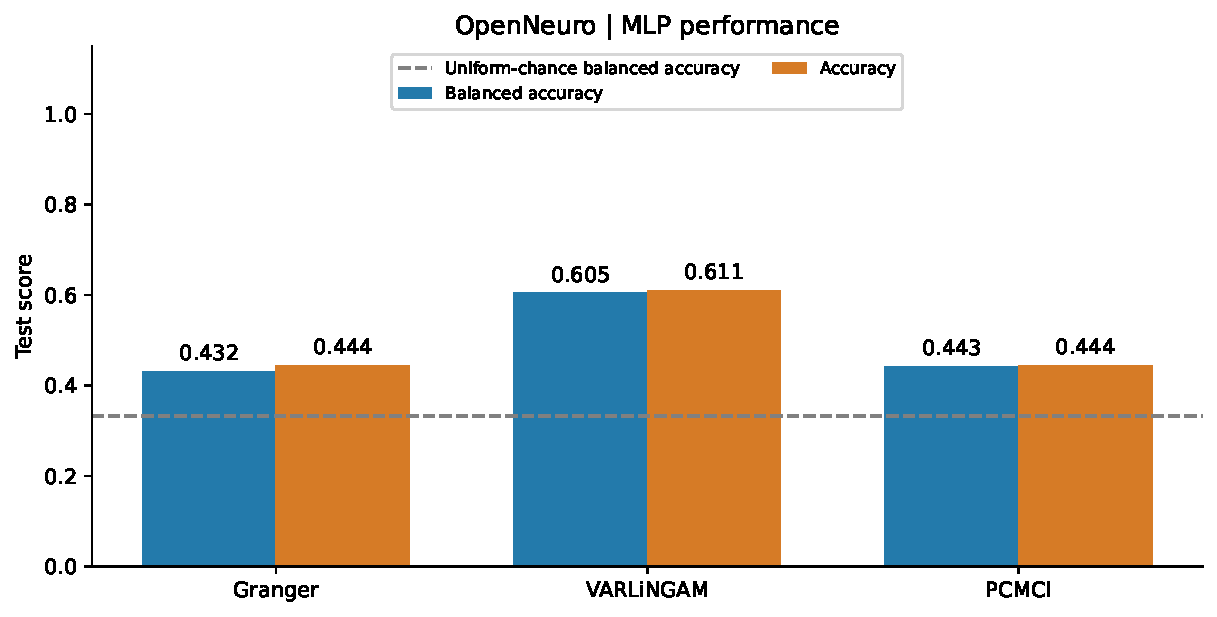
\includegraphics[width=\textwidth,height=0.32\textheight,keepaspectratio]{figures/mlp_openneuro_performance.pdf}
\caption{OpenNeuro: MLP test scores by connectivity method.}
\end{figure}
\begin{figure}[H]
\centering
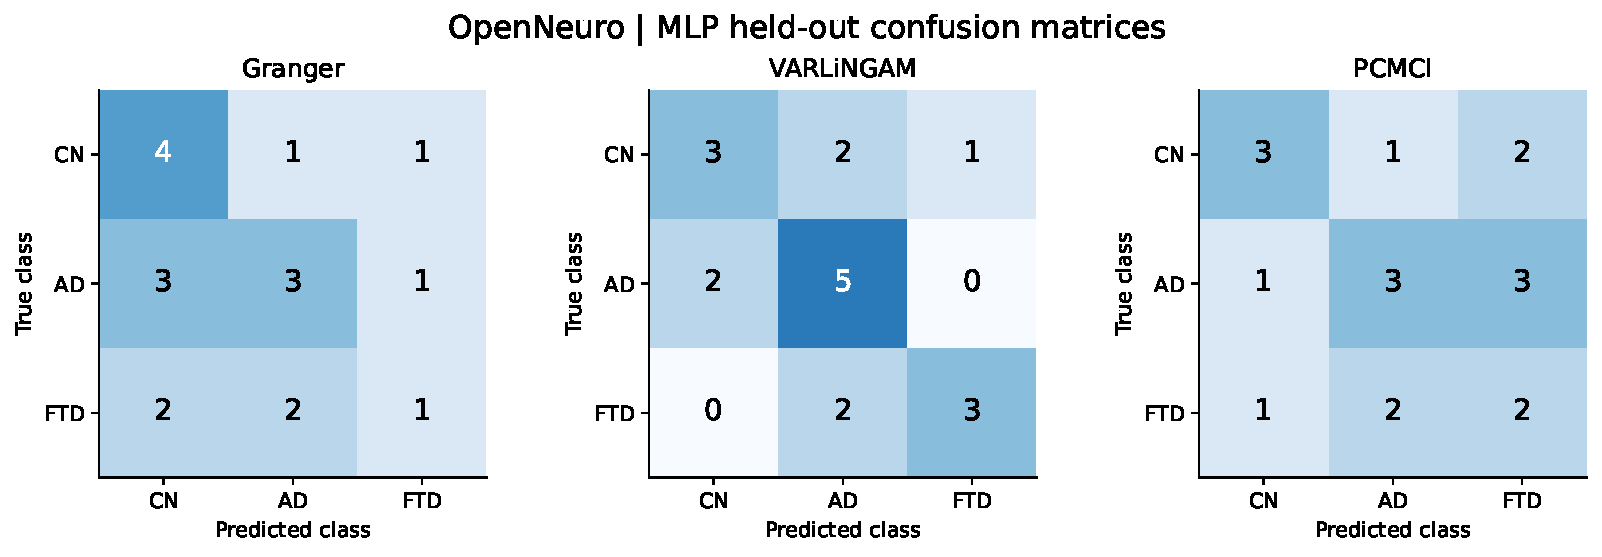
\includegraphics[width=\textwidth,height=0.28\textheight,keepaspectratio]{figures/mlp_openneuro_confusion.pdf}
\caption{OpenNeuro: test confusion matrices; true classes on rows and predictions on columns.}
\end{figure}

\subsection{BrainLat: independent within-dataset evaluation}
The split contains 59 training, 8 validation and 18 test subjects. Test support is 7 CN, 7 AD and 4 FTD.
\begin{table}[H]
\centering\small
\begin{tabular}{lllll}
\toprule
Adjacency & Balanced accuracy & Accuracy & Best epoch & Epochs run \\
\midrule
Granger & 0.821 & 0.833 & 6 & 56 \\
VARLiNGAM & 0.821 & 0.833 & 14 & 64 \\
PCMCI & 0.607 & 0.667 & 9 & 59 \\
\bottomrule
\end{tabular}
\caption{BrainLat: saved MLP test results, seed 42.}
\end{table}
\begin{figure}[H]
\centering
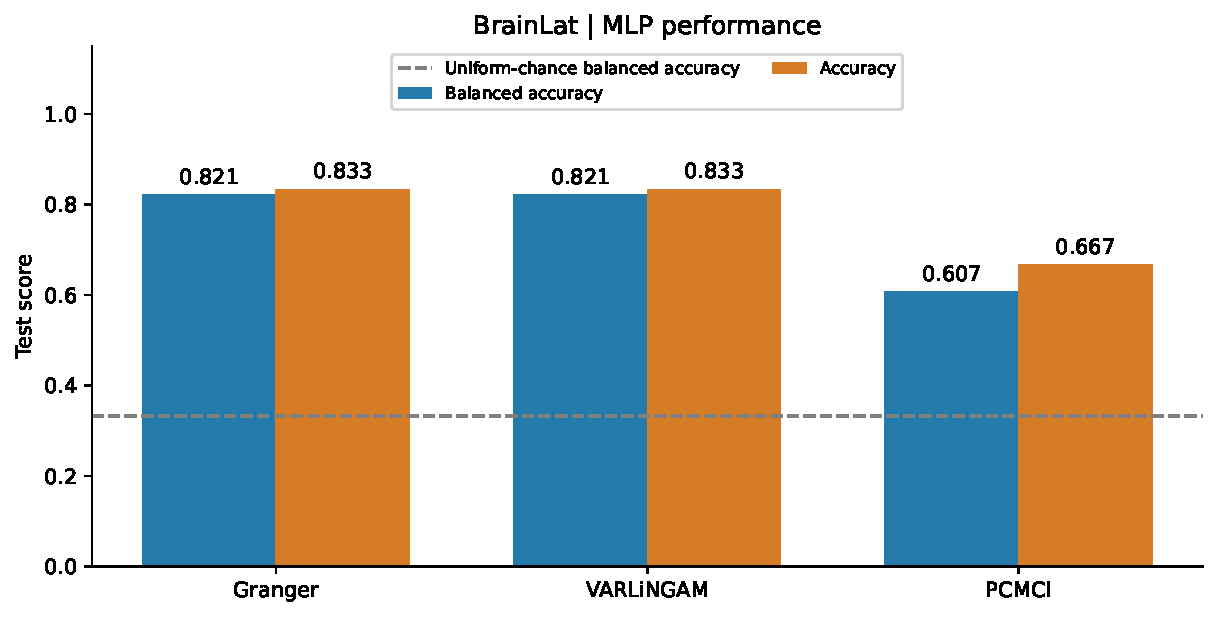
\includegraphics[width=\textwidth,height=0.32\textheight,keepaspectratio]{figures/mlp_brainlat_performance.pdf}
\caption{BrainLat: MLP test scores by connectivity method.}
\end{figure}
\begin{figure}[H]
\centering
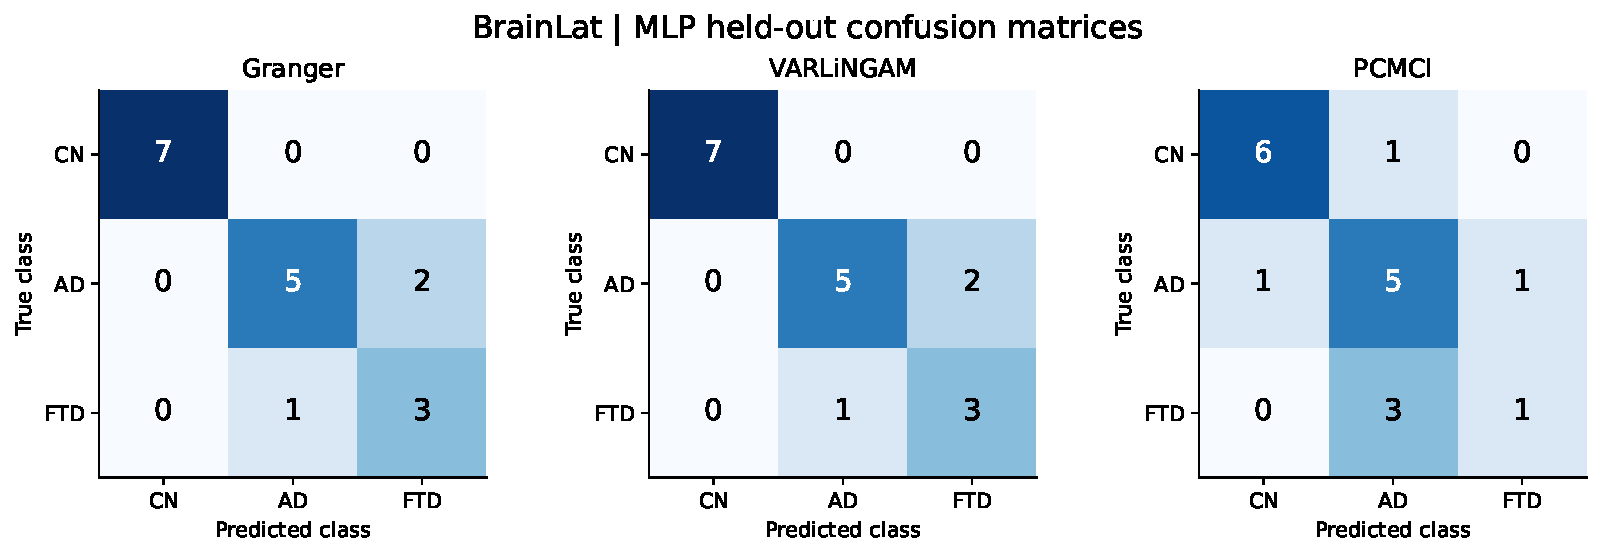
\includegraphics[width=\textwidth,height=0.28\textheight,keepaspectratio]{figures/mlp_brainlat_confusion.pdf}
\caption{BrainLat: test confusion matrices; true classes on rows and predictions on columns.}
\end{figure}

% END AUTO CLASSIFICATION

\subsection{Interpretation and scope}

% BEGIN AUTO MLP_INTERPRETATION
\paragraph{OpenNeuro.}
The independent run uses seed 42.
Granger obtains balanced accuracy 0.432 and accuracy 0.444 (8 of 18 correct). CN, AD and FTD recalls are 0.667, 0.429 and 0.200. The best validation loss is 0.503 at epoch 16 of 66 executed epochs.
VARLiNGAM obtains balanced accuracy 0.605 and accuracy 0.611 (11 of 18 correct). CN, AD and FTD recalls are 0.500, 0.714 and 0.600. The best validation loss is 0.421 at epoch 20 of 70 executed epochs.
PCMCI obtains balanced accuracy 0.443 and accuracy 0.444 (8 of 18 correct). CN, AD and FTD recalls are 0.500, 0.429 and 0.400. The best validation loss is 0.682 at epoch 4 of 54 executed epochs.
On OpenNeuro, VARLiNGAM achieves the highest observed test balanced accuracy (0.605).

The confusion matrices show that VARLiNGAM correctly identifies 3 of 6 CN,
5 of 7 AD and 3 of 5 FTD test subjects. Granger and PCMCI each classify
8 of 18 subjects correctly, but PCMCI has a slightly higher balanced
accuracy because the class recalls differ. FTD recall is 0.200 for
Granger, 0.600 for VARLiNGAM and 0.400 for PCMCI. All three observed
balanced accuracies exceed the uniform-chance reference of $1/3$;
this comparison alone is not a statistical significance test.

\paragraph{BrainLat.}
The independent run uses seed 42.
Granger obtains balanced accuracy 0.821 and accuracy 0.833 (15 of 18 correct). CN, AD and FTD recalls are 1.000, 0.714 and 0.750. The best validation loss is 0.940 at epoch 6 of 56 executed epochs.
VARLiNGAM obtains balanced accuracy 0.821 and accuracy 0.833 (15 of 18 correct). CN, AD and FTD recalls are 1.000, 0.714 and 0.750. The best validation loss is 0.476 at epoch 14 of 64 executed epochs.
PCMCI obtains balanced accuracy 0.607 and accuracy 0.667 (12 of 18 correct). CN, AD and FTD recalls are 0.857, 0.714 and 0.250. The best validation loss is 0.758 at epoch 9 of 59 executed epochs.
On BrainLat, Granger and VARLiNGAM tie for the highest observed test balanced accuracy (0.821).

Granger and VARLiNGAM produce identical test confusion matrices: both
correctly classify all 7 CN subjects, 5 of 7 AD subjects and 3 of 4 FTD
subjects. Their three errors consist of two AD subjects predicted as FTD
and one FTD subject predicted as AD. PCMCI correctly classifies 12 of 18
subjects, including only 1 of 4 FTD subjects; the remaining three FTD
subjects are predicted as AD. The different validation losses of Granger
and VARLiNGAM therefore do not imply different held-out classification
performance in this run.
% END AUTO MLP_INTERPRETATION

These are independent within-dataset experiments, not training on one
dataset and testing on the other. The better BrainLat scores do not isolate
a dataset effect: cohorts, acquisition conditions, retained durations and
test subjects differ. There are only 18 test subjects in each run; one
additional correct prediction changes accuracy by 5.6 percentage points.
No confidence intervals or paired significance tests are reported, and the
observed method ranking is not a validated model-selection result.

The experiments use node features and adjacency jointly. Without feature-only
and adjacency-only ablations, they do not quantify the incremental value of
connectivity. Repeated subject-level splits and external-dataset testing are
needed to assess robustness and transferability.

\section{Output Artifacts}

Each processed subject directory contains:
\begin{itemize}
    \item \texttt{X.npy}: node-feature matrix with shape $19\times8$;
    \item \texttt{preprocessed\_epochs.npy}: stationarized epochs used for
          causal estimation;
    \item six adjacency files, three directed and three symmetric;
    \item \texttt{y.json}: numerical and textual label;
    \item \texttt{metadata.json}: sampling rate, epoch count, channel count,
          feature count, and quality-control summary.
\end{itemize}
At dataset level, \texttt{summary.csv}, \texttt{config.json},
\texttt{splits.json}, and \texttt{graphs.pkl} provide traceability and
reproducibility.

\section{Limitations and Future Work}

The EEG-to-graph pipeline and classification experiments have several
methodological and experimental limitations.

First, the stationarity criterion is strict because it requires agreement
between ADF and KPSS. Future ablations should compare the current rule against
ADF-only stationarity or a rule that differences only when both tests indicate
non-stationarity. Second, each subject is summarized by a static graph even
though EEG connectivity is dynamic. Third, the number of subjects is small for
training high-capacity models, especially in the FTD class. Fourth, the
connectivity estimates are statistical and may be affected by latent sources,
volume conduction, unmodeled nonlinear effects, and multiple testing.

The natural next step is to train graph neural models using the method-specific
adjacency matrices, comparing directed and symmetric variants and reporting
ablation studies for node features, Granger, VARLiNGAM, and PCMCI. The current
MLP results provide a subject-level baseline for that stage.

\section{Conclusion}

The project represents EEG recordings as subject-level graphs combining
spectral and statistical node features with method-specific directed
connectivity. Granger causality, VARLiNGAM, and PCMCI provide complementary
representations for connectivity analysis and classification.
% BEGIN AUTO MLP_CONCLUSION
On OpenNeuro, VARLiNGAM achieves the highest observed test balanced accuracy (0.605).
On BrainLat, Granger and VARLiNGAM tie for the highest observed test balanced accuracy (0.821).
% END AUTO MLP_CONCLUSION
Dataset-specific connectivity figures preserve the distinction
between the two cohorts. The results remain preliminary and require
validation across repeated splits and independent cohorts.

\end{document}
